\documentclass[a4paper,11pt]{article}
\usepackage[top=23mm,bottom=23mm,left=25mm,right=25mm,footskip=10mm]{geometry}
\usepackage{lmodern,amsmath,amssymb,booktabs,graphicx,xcolor}
\usepackage{hyperref}
\definecolor{linkink}{HTML}{215368}
\hypersetup{colorlinks=true,linkcolor=linkink,citecolor=linkink,urlcolor=linkink,
  pdftitle={Counting three-column binary matrices with row and column sums at most two},
  pdfsubject={A combinatorial proof of the three-column formula in OEIS A401159, verified in Lean 4},
  pdflang={en}}
\newcommand{\ident}[1]{\texttt{\detokenize{#1}}}
\newcommand{\entrylink}{https://github.com/oeis/oeisdata/blob/b460c2e8ffbef9a3aacf263819282712f0f30341/seq/A401/A401159.seq}
\setlength{\emergencystretch}{1em}
% Both editions use the same theorem and the same seven published data points.
\newcommand{\threeColumnIdentities}{%
\begin{align}
 T(n,3) &= \left(1+n+\binom n2\right)^3-n^4+\binom n2 \label{eq:count}\\
        &= \frac{n^6+3n^5+n^4+13n^3+22n^2+8n+8}{8}. \label{eq:polynomial}
\end{align}%
}

\newcommand{\threeColumnValues}{%
\begin{tabular}{@{}lrrrrrrr@{}}
\toprule
$n$      &3&4&5&6&7&8&9\\
$T(n,3)$ &265&1\,081&3\,481&9\,367&22\,009&46\,585&90\,811\\
\bottomrule
\end{tabular}%
}

\raggedbottom

\begin{document}
\begin{center}
  {\Large\bfseries Counting three-column binary matrices\\[2pt]
    with row and column sums at most two\par}
  \vspace{4pt}
  {\small November 25, 2026\quad$\cdot$\quad\href{https://github.com/nktkt/math/blob/main/research/mathar_three_columns/output/pdf/three-columns-ja.pdf}{Japanese edition}\par}
\end{center}
\smallskip

\noindent\textbf{Abstract.}\quad
We count labeled $n\times3$ binary matrices with at most two ones in each row and
each column. Marking a row of three ones gives $n^4$ marked pairs. Exactly
$\binom n2$ matrices allow two choices of marked row. Correcting for this double
count gives the degree-six
polynomial conjectured by R.~J.~Mathar in OEIS A401159 for
every nonnegative $n$. We formalize this inclusion--exclusion proof in Lean~4.

\section{The counting problem}
Write $[n]=\{1,\ldots,n\}$, with $[0]=\varnothing$. Let $T(n,m)$ be the number of
binary matrices with $n$ labeled rows and $m$ labeled columns in which every row
sum and every column sum is at most two. Mathar gave a recurrence for general
dimensions and tabulated small cases \cite[Section~2 and Table~2]{mathar2014}.
In 2026 he recorded the polynomial in~\eqref{eq:polynomial} as a conjecture for
three columns \cite{oeis}.

\smallskip
\noindent\textbf{Theorem 1.}\quad For every integer $n\geq 0$,
\threeColumnIdentities

\section{Proof by column supports}
Let $S_j\subseteq[n]$ be the set of rows with a one in column $j$. A set of size
at most two can be chosen in $B=1+n+\binom n2$ ways. Choosing all three supports
independently gives $B^3$ matrices satisfying the column bounds. A row violates
its bound precisely when it belongs to all three supports. Put
$q=|S_1\cap S_2\cap S_3|$. Each support has size at most two, so $q\leq 2$.

Count pairs $(A,i)$ in which $A$ satisfies the column bounds and $i$ is a marked
row of three ones. For a fixed $i$, each column support is either $\{i\}$ or
$\{i,a\}$ for one of the $n-1$ other rows $a$. This gives $n$ choices per column,
and $n\cdot n^3=n^4$ marked pairs in all. If $q=2$, the two common rows force
each column support to equal the same pair. Each unordered pair of rows gives
exactly one such matrix, for a total of $\binom n2$.

Subtracting $n^4$ from $B^3$ removes each matrix with $q=1$ once and each matrix
with $q=2$ twice. Adding back the latter once gives~\eqref{eq:count}. Substitution
of $\binom n2=n(n-1)/2$ and expansion give~\eqref{eq:polynomial}. For $n=0$ both
sides count the unique empty matrix.\hfill$\square$

\begin{center}
  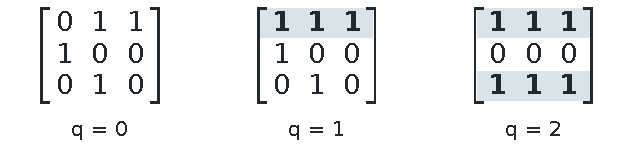
\includegraphics[width=.69\linewidth]{marked-rows.pdf}\par
  \smallskip
  {\small Figure 1. Shading marks rows of three ones. The rightmost matrix admits two choices of marked row.}
\end{center}

\newpage
\section{A derivation from the 2014 table}
The polynomial can also be recovered from Mathar's table once its degree is
bounded. Let $a_k$ count admissible $k\times3$ matrices whose rows are all
nonzero, with $a_0=1$. The three columns contain at most six ones altogether,
so a matrix can have at most six nonzero rows.

Deleting the zero rows of a matrix with $k$ nonzero rows gives an object counted
by $a_k$. Conversely, choosing a $k$-element subset of $[n]$ specifies where to
put these rows, in order, and thus recovers the original matrix. Consequently,
\begin{equation}
 T(n,3)=\sum_{k=0}^{6} a_k\binom nk . \label{eq:basis}
\end{equation}
Here $\binom nk=0$ when $n<k$. For fixed $k$, $\binom nk$ is a polynomial in
$n$ of degree $k$ over the rationals. Thus $T(n,3)$ agrees with a polynomial of
degree at most six on the nonnegative integers.

\begin{center}
{\small Table 1. The three-column entries from Mathar's Table~2 \cite{mathar2014}.}\par
\smallskip
\threeColumnValues
\end{center}

Evaluating the right-hand side of~\eqref{eq:polynomial} at $n=3,\ldots,9$ gives
the seven values in Table~1. Two polynomials of degree at most six that agree
at these seven distinct arguments are equal. This gives a second proof using
the tabulated values and~\eqref{eq:basis}. The OEIS entry consulted on
November~25, 2026 labels the three-column formula a conjecture \cite{oeis}.
The historical priority of a proof remains undetermined.

\section{Formalization in Lean 4}
A binary matrix has type \ident{Fin n} $\to$ \ident{Fin m} $\to$ \ident{Bool}.
For each row and each column, the predicate \ident{Admissible} bounds by two the
cardinality of its set of true entries. The cardinality of the subtype of matrices
satisfying this predicate defines \ident{T n m}. Passing to three supports uses
an explicit equivalence. Taking supports is the forward map, and testing
membership in a support recovers each entry.

The theorem \ident{count_three_columns} proves~\eqref{eq:count} over the natural
numbers in the form
\[
 T(n,3)+n^4=\left(1+n+\binom n2\right)^3+\binom n2.
\]
The theorem \ident{mathar_A401159_three_columns} casts this equality to the
rationals and expands the binomial coefficient to obtain Mathar's formula.
The proof was checked with Lean 4.29.1. The
\href{https://github.com/nktkt/math/tree/main/research/mathar_three_columns}{accompanying repository} contains the pinned
mathlib revision, the verification commands, and a check of the displayed
polynomial directly against the type of admissible Boolean matrices.

\begin{thebibliography}{9}
\bibitem{mathar2014}
Richard J. Mathar.
\emph{The number of binary $n\times m$ matrices with at most $k$ 1's in each row or column}.
November 23, 2014. \href{https://oeis.org/A247158/a247158.pdf}{Manuscript}.
\bibitem{oeis}
Richard J. Mathar. \emph{OEIS A401159}. The On-Line Encyclopedia of Integer Sequences,
revision 9, November 18, 2026. \href{https://oeis.org/A401159}{Entry}
and \href{\entrylink}{archived revision}.
\end{thebibliography}
\end{document}
